\documentclass[10pt,a4paper]{article}
\usepackage{fontspec}
\usepackage[slantfont, boldfont]{xeCJK}
\usepackage{graphicx}

\XeTeXlinebreaklocale "zh"
\XeTeXlinebreakskip = 0pt plus 1pt minus 0.1pt

\setCJKmainfont{Adobe Heiti Std}
%\parindent 2em

\begin{document}
\title{Improve the UI of Voici Image Processor}
\author{Song Wenhao}
\date{\today}
\maketitle
\section{Toolbar Buttons}
Add icons to the toolbar buttons, to make them easier to recognize.\\

Origin:\\
\indent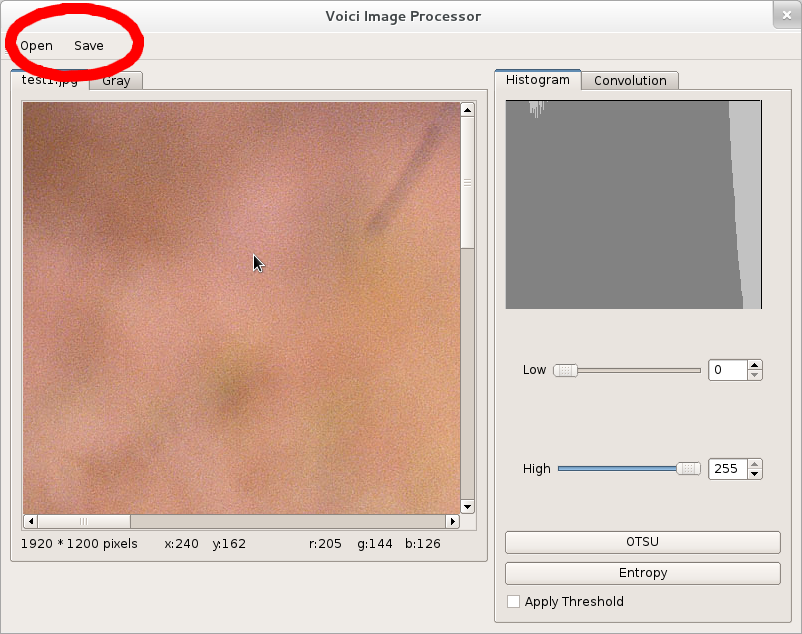
\includegraphics[width=0.65\textwidth]{icon_origin.png}\\

Improved:\\
\indent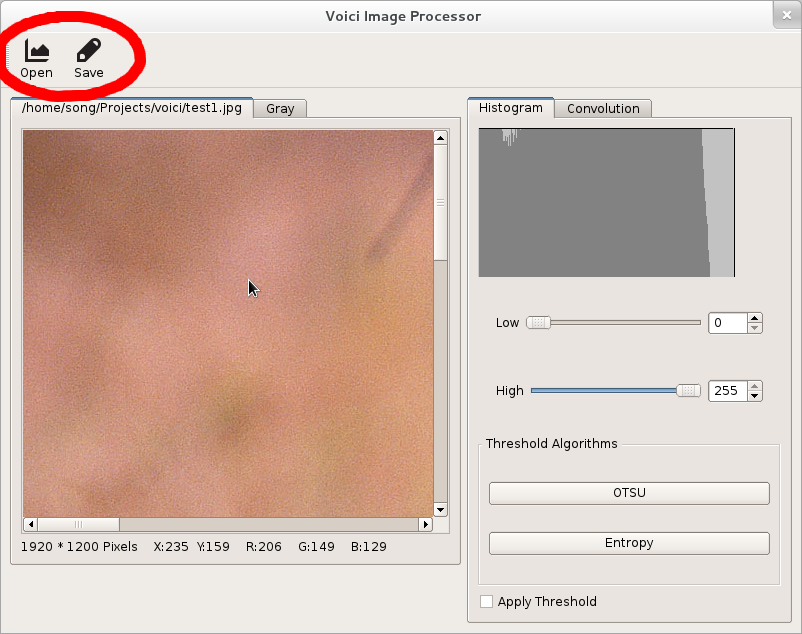
\includegraphics[width=0.65\textwidth]{icon_improved.png}

\pagebreak


\section{Groups}
Make buttons of similar functions together, and those of different functions apart.\\

Origin:\\
\indent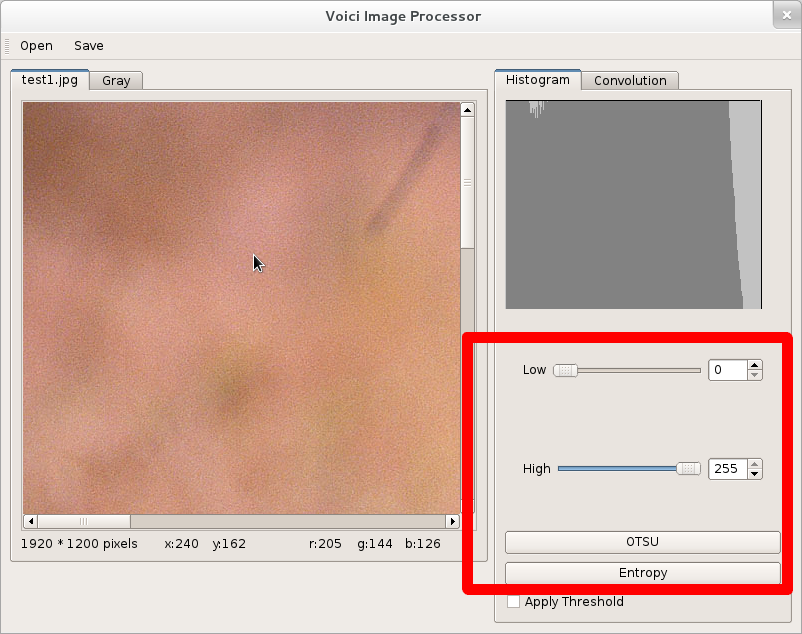
\includegraphics[width=0.65\textwidth]{group_origin.png}\\

Improved:\\
\indent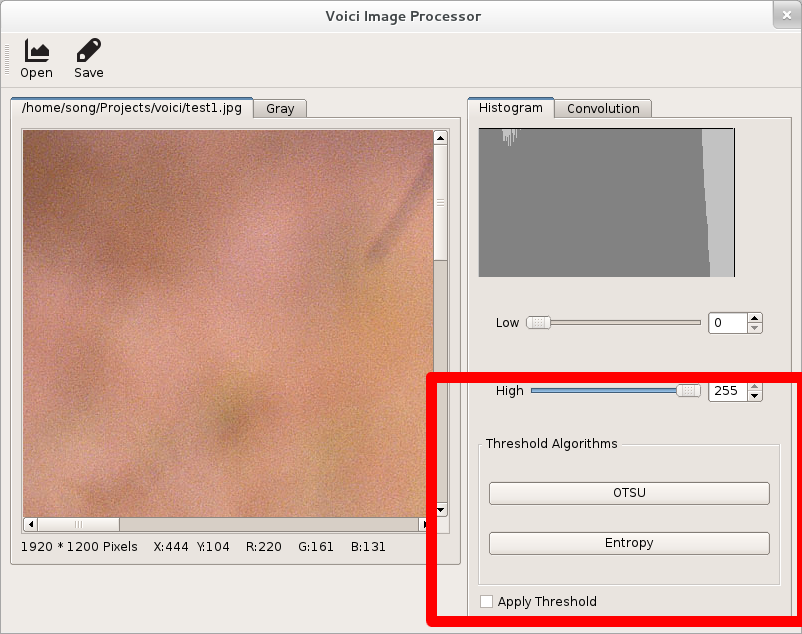
\includegraphics[width=0.65\textwidth]{group_improved.png}

\pagebreak

\section{Kernel Center Color}
Change the color of the table item, to give the user a direct idea of which item he chooses for the kernel center.\\

Origin:\\
\indent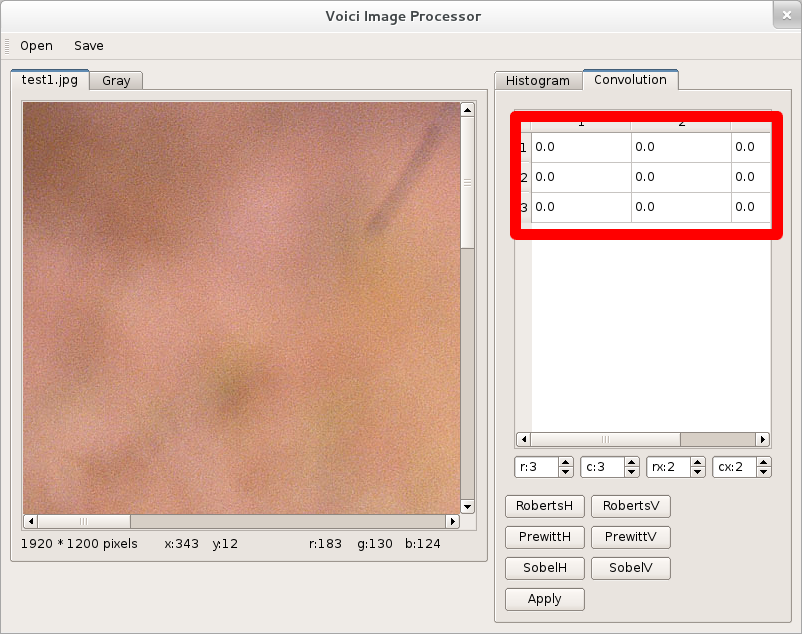
\includegraphics[width=0.65\textwidth]{item_origin.png}\\

Improved:\\
\indent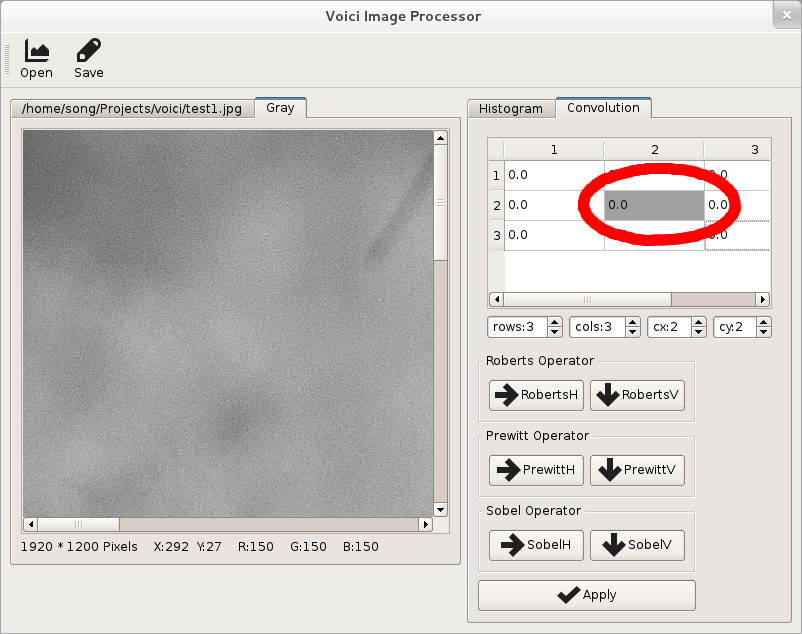
\includegraphics[width=0.65\textwidth]{item_improved.png}

\pagebreak

\section{Button Groups}
Make buttons of the same class together. Use icon to give the user an quick idea of difference of buttons within the same class.\\

Origin:\\
\indent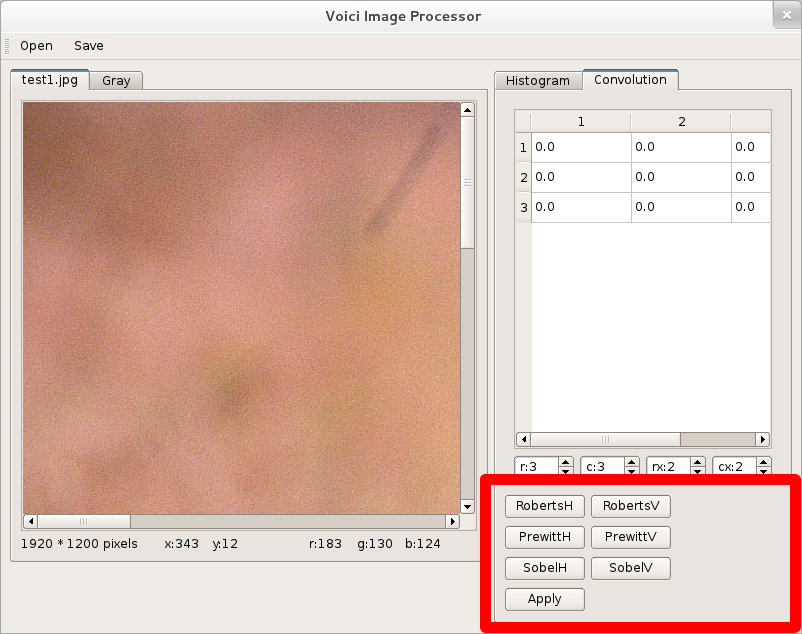
\includegraphics[width=0.65\textwidth]{icon_and_group_origin.png}\\

Improved:\\
\indent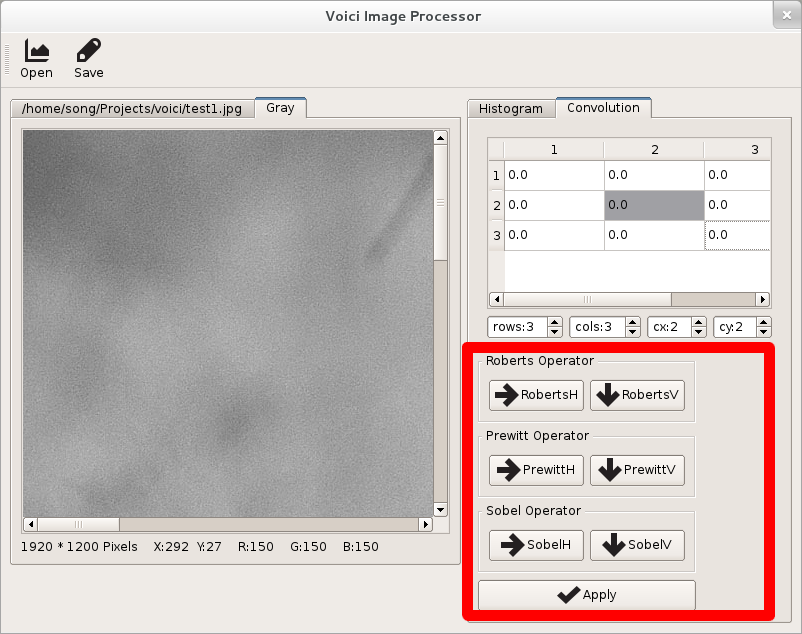
\includegraphics[width=0.65\textwidth]{icon_and_group_improved.png}

\pagebreak

\section{Cursor}
In the improved version, the cursor will become a cross when the mouse moves to the image.

Because the screen snapshoot tool on my computer doesn't take the pointer effect, into the picture, you can try this improvement yourself.

\section{Internationalize}
Make a Chinese version on the English version. This makes the software easier to understand by users of different languages.\\

Improved:\\
\indent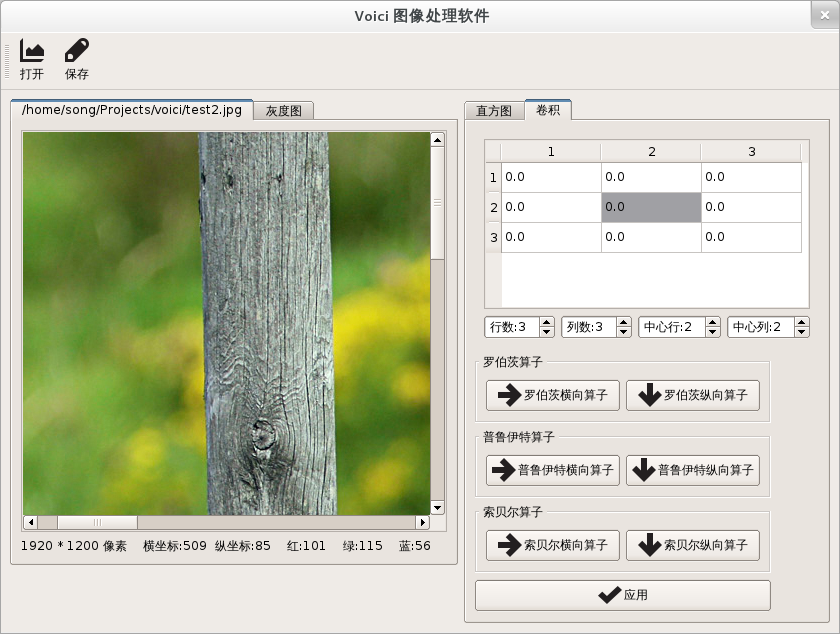
\includegraphics[width=0.65\textwidth]{chinese_improved.png}

\section{Why not change the UI color}
I think the default one is good enough. It is not cool, but the users will not feel uncomfortable with their eyes. I think the pratical reason is more important.

\end{document}


